% On the other hand, assuming purely rigid motions is a strong restriction that is barely fulfilled in organic shapes. When a person moves, there are parts of their body moving rigidly (e.g. upper and lower arms or legs) and others which are transitions between the rigid ones (e.g. the neck). Be- sides, rigid motions within a fine-grained articulated struc- ture may not be observable with the limited resolution of a camera. For these reasons, a sharp segmentation will never be able to estimate the motion of life beings or some other inanimate objects with exactitude.

%TODO: think about where to explain the difference between rigid-and deformable motion.

% RELATED WORK - OF
%=> SRSF
%source 1:
% 
%propose    a    per-pixel    over-
%parameterized representation using rotation and translation
%to  capture  the  global  rigid  motion  of  the  scene  while
%allowing  local  deviations.    Their  method  is  more  suited
%for  a  single  moving  object.   By  comparison  our  method
%captures the global 3D motion for each individually moving
%object  and  can  handle  multiple  moving  objects
%source 2:
%
%overparametrize scene flow and estimate a 6-DoF rigid- body motion at each pixel. They regularize the flow field in this 6-DoF parametrization such that their model favors lo- cally rigid motions

\chapter{Introduction}
\section{Motivation}
In nature one important aspect that determines the odds of survival and thus the individual success is the ability to sense the surrounding environment. In particular, the perceptional system of any advanced species is directed by visual cues amongst others. Alongside with sensing color, depths and brightness, the perception of motion is a fundamental visual cue. Particularly, is of great importance for interpreting visual information such as object groupings and their structure, estimating speed and performing self-localization.
\begin{figure}[H]
\begin{center}
\subfigure[Frame 1]{
   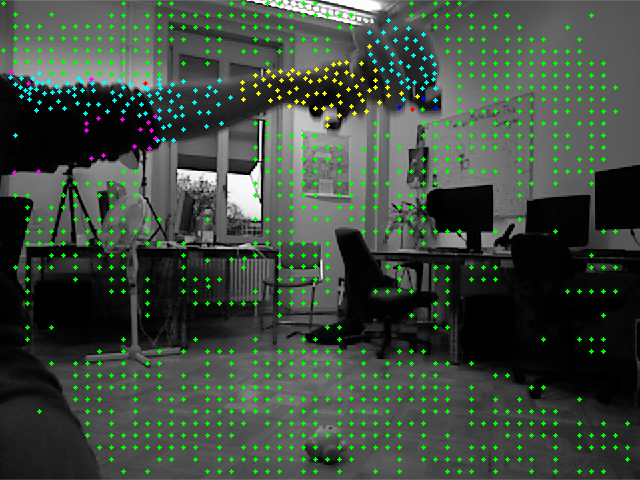
\includegraphics[width=0.31\linewidth] {evaluation/bonn_chairs_frames/1}
   \label{fig:motivating_example_a}
}
\subfigure[Frame 12]{
   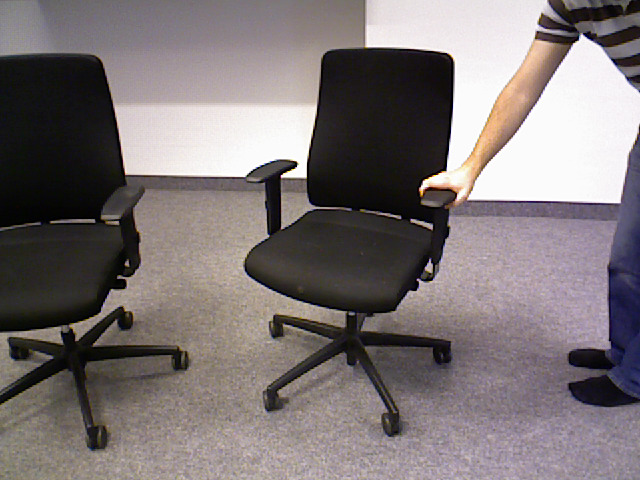
\includegraphics[width=0.31\linewidth] {evaluation/bonn_chairs_frames/12}
   \label{fig:motivating_example_b}
}
\subfigure[Frame 24]{
   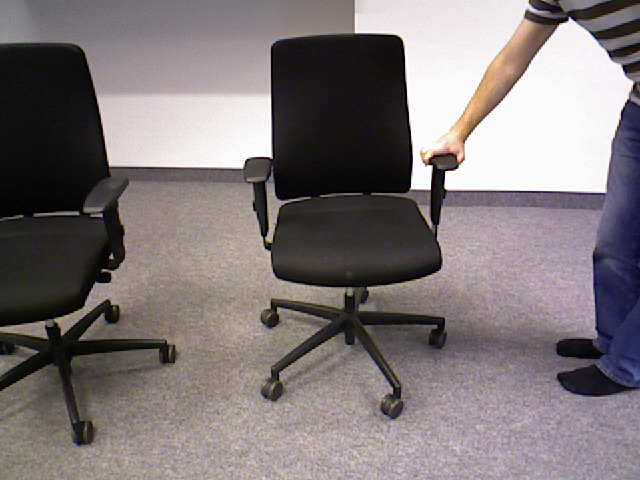
\includegraphics[width=0.31\linewidth] {evaluation/bonn_chairs_frames/24}
   \label{fig:motivating_example_c}
}
\end{center}
\caption[Motivating Example]{foobar}
\label{fig:motivating_example}
\end{figure}
As natural this tasks might be performed by our brains as hard it becomes to realize in a technical point of view. Especially the task of an accurate detection and extraction of the moving objects in a video, captured by a moving camera, is nowadays still an unresolved problem. \\ \\
However, a lot of scientific effort has been put into this problem statement and many sophisticated approaches have been established. In particular, the most promising motion segmentations were produced by methods relying on optical flows. An example is given in figure $\ref{fig:motion_segmentation_motivation_eg}$.
\begin{figure}[H]
\begin{center}
\subfigure[Optical Flow Field]{
   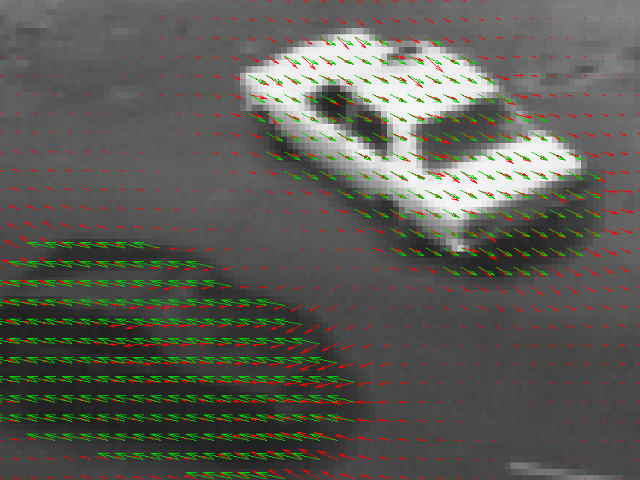
\includegraphics[width=0.47\linewidth] {introduction/motivation/motion_segmentation/optical_flow_visualization}
   \label{fig:motion_segmentation_motivation_eg_a}
}
\subfigure[Motion Segmentation]{
   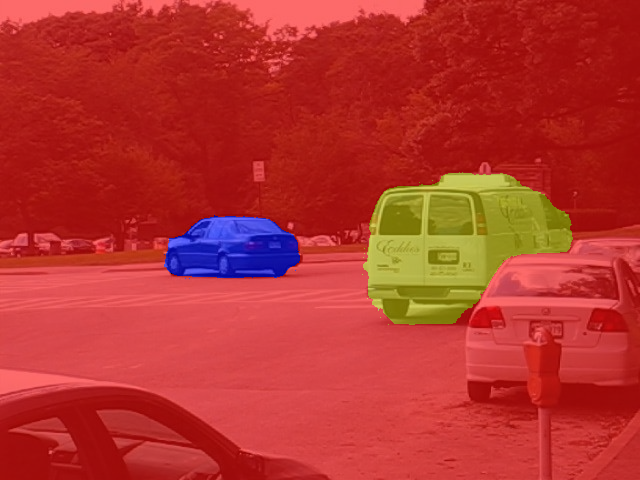
\includegraphics[width=0.47\linewidth] {introduction/motivation/motion_segmentation/dense_motion_segmentation}
   \label{fig:motion_segmentation_motivation_eg_b}
}
\end{center}
\caption[Motion Segmentation Motivation Example]{An example$\footnotemark$ of an optical flow field and a notion Segmentation. }
\label{fig:motion_segmentation_motivation_eg}
\end{figure}
\footnotetext{Source figure \ref{fig:motion_segmentation_motivation_eg_a}: \url{http://cbia.fi.muni.cz/projects/optical-flow-for-live-cell-imaging_3.html} \\
 and source figure\ref{fig:motion_segmentation_motivation_eg_b}: \url{http://lmb.informatik.uni-freiburg.de/research/segmentation/}}
The field of motion segmentation aims at decomposing a video in moving objects and background and s the first fundamental step in many computer vision algorithms. It has many applications in the fields of robotics, metrology, video surveillance, traffic monitoring. \\ \\
The idea of using optical flows as an estimate of the motion goes back to the pioneering work of B. Horn and B. Schunck $\cite{Hs81}$. In their recent work $\cite{KB15b}$, T. Brox et all published such a motion segmentation pipeline . \\ \\
An orthogonal technique to generate motion segmentation is to order the objects according to their depth layer. Unfortunately, this approach requires depth measurements of dataset frames. Until recently, measuring depths in videos was rather unpractical since it required dedicated and expensive capturing devices and additional post-processing. However, due to the success of Microsoft Xbox' Kinect, the competition among these capturing devices has increased and the prices became affordable. \\ \\
Idially, a motion segmentation pipeline would therefore make use of optical flows and the same time exploit measured depth maps. 

\section{Goals}
The purpose of this thesis is to describe a robust motion segmentation method
that uses RGB-D$\footnote{The term \textit{RGB-D} refers to color images with associated depth field measurements.}$ video sequences as well as other visual cues. In particular, our segmentation method should make use of optical flows. In our formulation we assume a piecewise rigid motion model and do not constrain the camera movement. \\ \\
The actual problem statement we want to address is shown in figure $\ref{fig:problem_statement}$. 
\begin{figure}[H]
\begin{center}
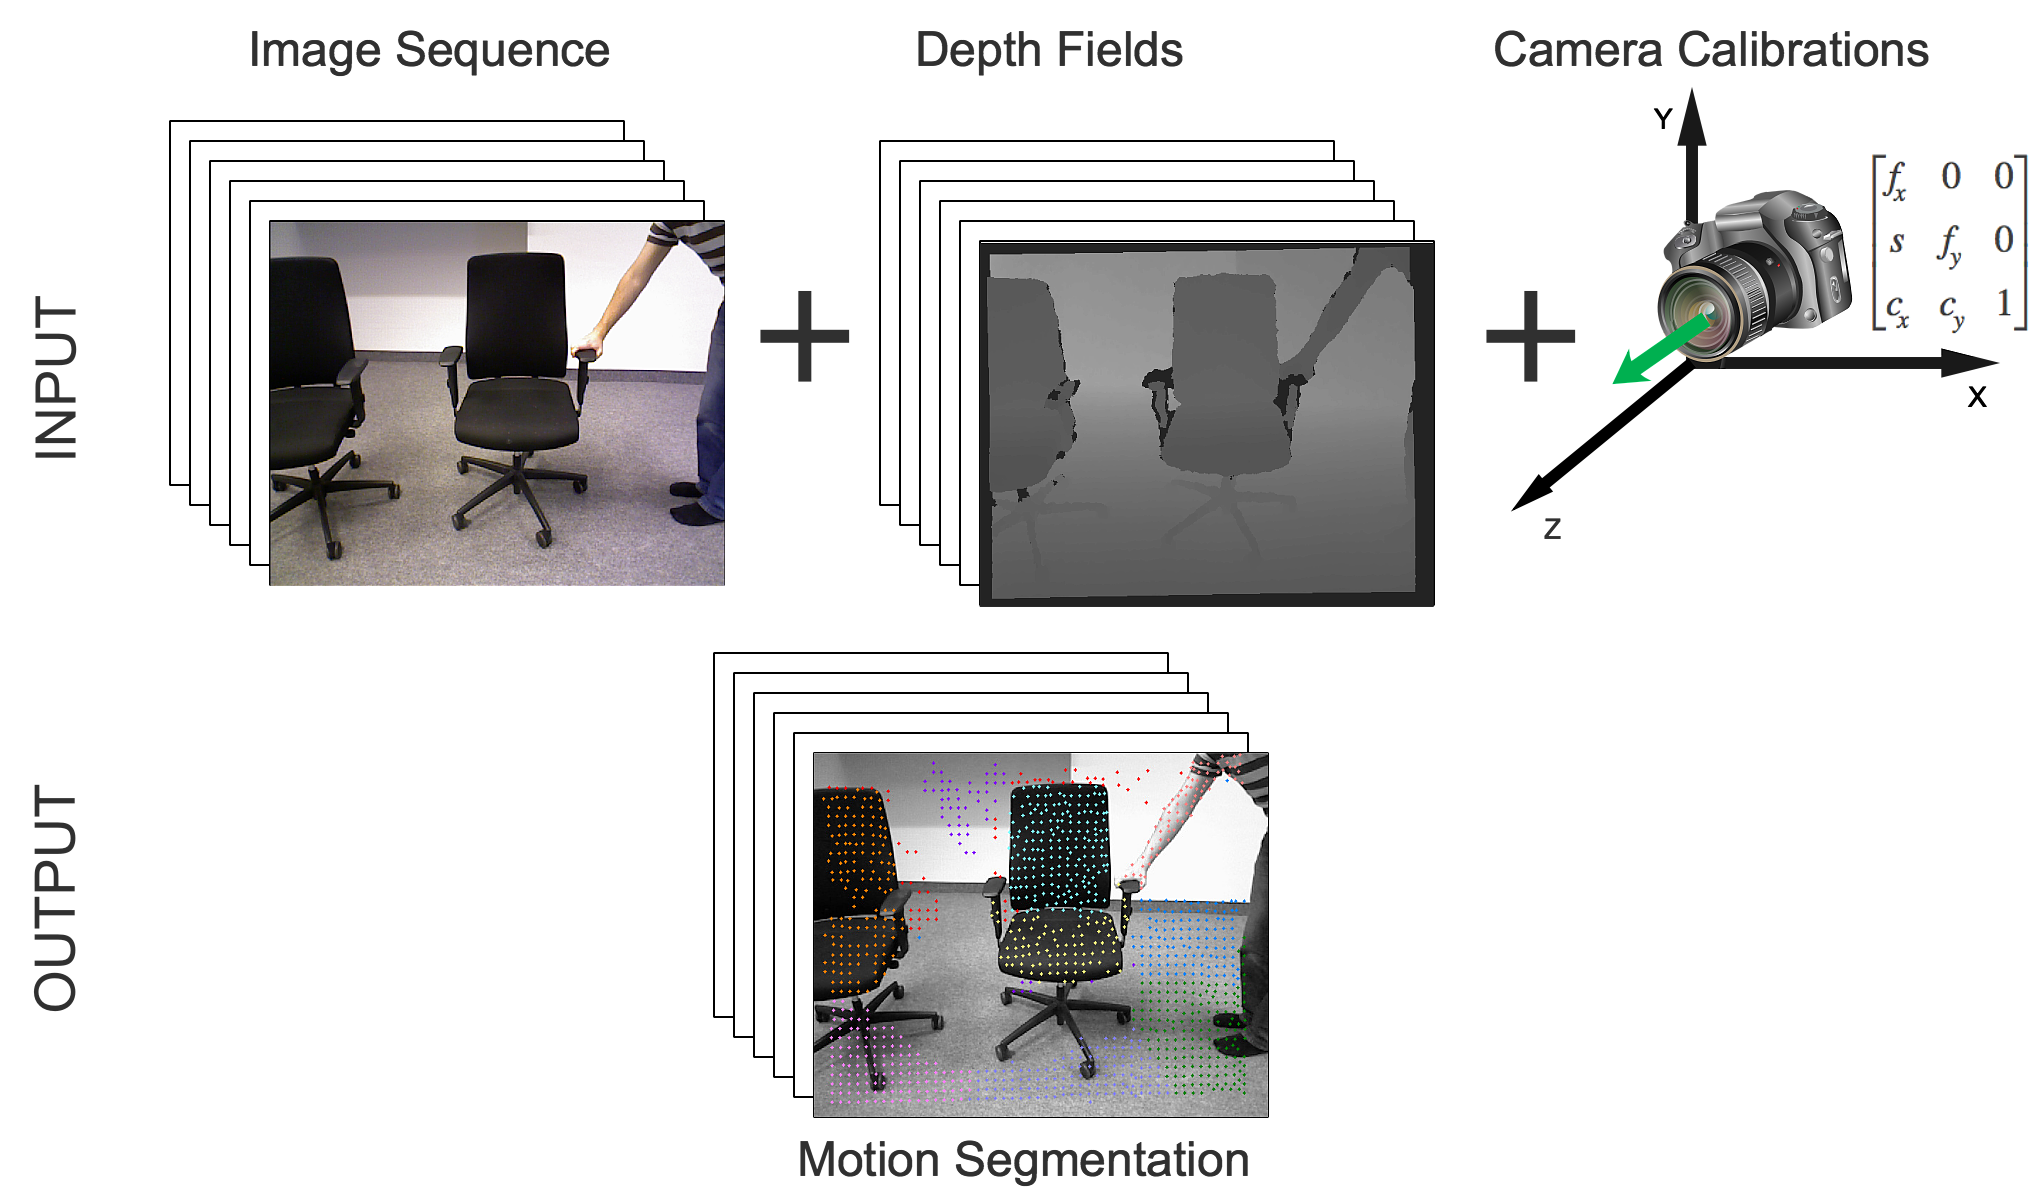
\includegraphics[width=1.05\linewidth] {introduction/problem_statement_ref}
\end{center}
\caption[Problem Statement]{ Graphical representation of the problem statement we want to solve in this thesis. Given a video sequence, its corresponding depth fields and the used camera calibrations, we want to extract the frames locations that mask the moving objects via segmentation.}
\label{fig:problem_statement}
\end{figure}
For a given RGB-D video sequence and the camera calibration data, we want to detect and extract the individual moving objects. We therefore develop a pipeline that is capable of generating such motion segmentations by using optical flows. \\ \\
Moreover, we want to examine the influence of the utilized pipeline components. Hence, we integrate various segmentation-and flow-techniques into our implementation. We then quantitatively evaluate segmentations generated by all possible pipeline combinations. \\ \\
In summary, we want to achieve the following three goals:
\begin{itemize}
  \item Implement a pipeline that can segment moving objects by running a long term analysis of point trajectories by using optical flows and depth cues.
  \item Examine the influence of the used flows, the method of trajectory analysis and segmentation and how they affect the segmentation quality by varying those components in the pipeline. For that purpose our pipeline implements various state of the art flow generation methods, different analysis approaches and a series of segmentation techniques.
  \item Quantitatively evaluate the resulting segmentation quality produced by running various pipeline combinations by comparing them against manually drawn ground truth segments.
\end{itemize}
Additionally, our implementation should be robust according to complex camera movement and noise, should be able to deal with occlusions and missing data and can handle many moving objects. \\ \\

\section{Related Work}
In this thesis we encounter and use many concepts from various fields. In particular we have deal with optical flow estimation methods, motion tracking analysis techniques and different segmentation concepts. In the following we give a brief summary of related work, state which parts are common with respect to our implementation and lastly, we state our contribution.

\subsection{Optical Flow}
list various existing methods to compute the optical flow

a vector motion field which describes the distribution of the apparent velocities of brightness patterns in a sequence. 

first formalized and computed  for  image  sequences  by  Horn  and  Schunck $\cite{Hs81}$ in  the  1980. Since the pioneering work of Horn and Schunck, many other approaches have been proposed:

\subsection{Motion Segmentation}
In this section we describe different approaches that can be used to address the task of motion segmentation.

\paragraph{Image Difference:} Taking the difference between two frames is a simple technique for detecting changes. By thresholding the intensity difference of two frames, a coarse map of the temporal changes can be obtained. Despite its simplicity, this techniques is limited by the presence of noise, camera movement (everything is changing) and low frame rates (nothing is changing). However, instead of directly using the difference image as the segmentation, the rough map of the changing areas can be used as a guide to extract spatial or temporal information in order to track the regions. Image difference techniques have been used in the work of $\cite{Cav05}$, $\cite{Li07}$ and $\cite{Col07}$.

\paragraph{Statistical Approach} Motion segmentation can be related to a classification problem, identifying whether a particular pixel belongs to either the background or the foreground. In $\cite{Cre05}$ the authors present a variational approach for segmenting an image into a set of regions of parametric motions using a model based on a conditional probability for the spatio-temporal image gradient. By exploiting Bayesian theory, they derive a cost functional which depends on parametric motion models for each  of a set of regions and on the boundary separating these regions.

\paragraph{Wavelets}
The idea is to exploit the ability of wavelets to perform analysis of the different frequency components of the images and then study each component with a resolution matched to its scale. Usually wavelet multi-scale decomposition is used in order to reduce the noise and in conjunction with other approaches, such as optical flow.

\paragraph{Layer Based} The key idea of layers based techniques is to understand which are the different depth layers in the image and which objects lie on which layer. 

\paragraph{Factorization Methods} Allow to recover the structure and motion by using traced features over a the whole image sequence.

\paragraph{Optical Flow}
track features using the optical flow over the given image sequence, compute affinity matrix based on similarity between the overlapping trajectories, use affinity matrix as an input to solve the segmentation task. LIST work but only shallow and briefly

$\cite{Bro11a}$

\section{Thesis Structure}

The reminder of this thesis is organized as follows:
In chapter 2 we start by providing the reader the relevant background in order to following the later chapters of this thesis. This chapter gives a detailed introduction to the concept of optical flow, to segmentation, spectral clustering and graph cut. It also explains how motion segmentation using optical flow is usually approached. \\ \\
In chapter 3 we develope all relevant derivations used to implemented the final pipeline. \\ \\
In chapter 4 we describe the implementation of our motion segmentation pipeline and all its stages in detail. \\ \\
In chapter 5 we list and discuss the results of some performed experiments. We start by introducing the reader to our used datasets. In our experiments section, we perform a qualitative-, as well as a quantitative evaluation. We explore the impact of the huge parameter-space due to the various stages of the implemented pipeline. Last, we also show some good segmentations, using the best (greedy found) parameters on our datasets. \\ \\
And finally Chapter 6 contains the conclusion of this thesis discussing what has been achieved in this thesis and the drawbacks of the proposed method. It also contains a note about some of my personal experiences during this thesis. 